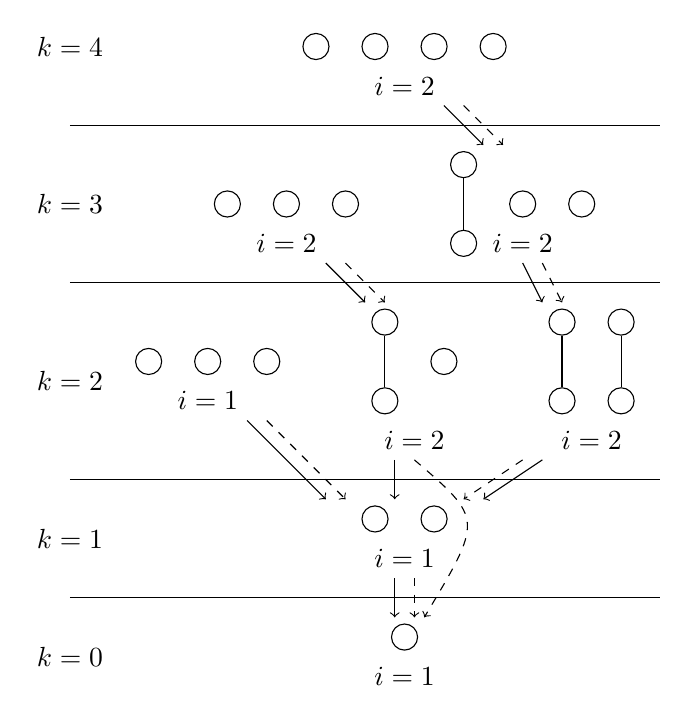
\begin{tikzpicture}

  % Level k = 4
  \node at (-1, 8) {$k=4$};

  \node[circle,draw=black] (k4_1) at (2.125 + 0 * 0.75, 8) {};
  \node[circle,draw=black] (k4_2) at (2.125 + 1 * 0.75, 8) {};
  \node[circle,draw=black] (k4_3) at (2.125 + 2 * 0.75, 8) {};
  \node[circle,draw=black] (k4_4) at (2.125 + 3 * 0.75, 8) {};
  \node at (2.125 + 0.75 * 1.5, 7.5) {$i=2$};

  \draw[->, dashed] (4, 7.25) -- (4.5, 6.75);
  \draw[->] (3.75, 7.25) -- (4.25, 6.75);

  \draw (-1, 7) -- (6.5, 7);

  % Level k = 3
  \node at (-1, 6) {$k=3$};

  \node[circle,draw=black] (k3_1) at (1 + 0 * 0.75, 6) {};
  \node[circle,draw=black] (k3_2) at (1 + 1 * 0.75, 6) {};
  \node[circle,draw=black] (k3_3) at (1 + 2 * 0.75, 6) {};
  \node at (1 + 0.75, 5.5) {$i=2$};

  \draw[->, dashed] (2.5, 5.25) -- (3, 4.75);
  \draw[->] (2.25, 5.25) -- (2.75, 4.75);

  \node[circle,draw=black] (k3_4) at (4 + 0 * 0.75, 6.5) {};
  \node[circle,draw=black] (k3_5) at (4 + 0 * 0.75, 5.5) {};
  \node[circle,draw=black] (k3_6) at (4 + 1 * 0.75, 6) {};
  \node[circle,draw=black] (k3_7) at (4 + 2 * 0.75, 6) {};
  \draw (k3_4) -- (k3_5);
  \node at (4 + 0.75, 5.5) {$i=2$};

  \draw[->, dashed] (5, 5.25) -- (5.25, 4.75);
  \draw[->] (4.75, 5.25) -- (5, 4.75);

  \draw (-1, 5) -- (6.5, 5);

  % Level k = 2
  \node at (-1, 3.75) {$k=2$};

  \node[circle,draw=black] (k2_1) at (0 + 0 * 0.75, 4) {};
  \node[circle,draw=black] (k2_2) at (0 + 1 * 0.75, 4) {};
  \node[circle,draw=black] (k2_3) at (0 + 2 * 0.75, 4) {};
  \node at (0 + 0.75, 3.5) {$i=1$};

  \draw[->, dashed] (1.5, 3.25) -- (2.5, 2.25);
  \draw[->] (1.25, 3.25) -- (2.25, 2.25);

  \node[circle,draw=black] (k2_4) at (3 + 0 * 0.75, 3.5) {};
  \node[circle,draw=black] (k2_5) at (3 + 0 * 0.75, 4.5) {};
  \node[circle,draw=black] (k2_6) at (3 + 1 * 0.75, 4) {};
  \draw (k2_4) -- (k2_5);
  \node at (3 + 0.75 * 0.5, 3) {$i=2$};

  \draw[->, dashed] (3.375, 2.75) .. controls (4.25, 2) .. (3.5, 0.75);
  \draw[->] (3.125, 2.75) -- (3.125, 2.25);

  \node[circle,draw=black] (k2_7) at (5.25 + 0 * 0.75, 3.5) {};
  \node[circle,draw=black] (k2_8) at (5.25 + 0 * 0.75, 4.5) {};
  \node[circle,draw=black] (k2_9) at (5.25 + 1 * 0.75, 3.5) {};
  \node[circle,draw=black] (k2_10) at (5.25 + 1 * 0.75, 4.5) {};
  \draw (k2_7) -- (k2_8);
  \draw (k2_9) -- (k2_10);
  \node at (5.25 + 0.75 * 0.5, 3) {$i=2$};

  \draw[->, dashed] (4.75, 2.75) -- (4, 2.25);
  \draw[->] (5, 2.75) -- (4.25, 2.25);

  \draw (-1, 2.5) -- (6.5, 2.5);

  % Level k = 1
  \node at (-1, 1.75) {$k=1$};

  \node[circle,draw=black] (k1_1) at (2.875 + 0 * 0.75, 2) {};
  \node[circle,draw=black] (k1_2) at (2.875 + 1 * 0.75, 2) {};
  \node at (2.875 + 0.75 * 0.5, 1.5) {$i=1$};

  \draw[->, dashed] (3.375, 1.25) -- (3.375, 0.75);
  \draw[->] (3.125, 1.25) -- (3.125, 0.75);

  \draw (-1, 1) -- (6.5, 1);

  % Level k = 0
  \node at (-1, 0.25) {$k=0$};

  \node[circle,draw=black] (k0_1) at (3.25, 0.5) {};
  \node at (3.25, 0) {$i=1$};
\end{tikzpicture}
